
\section{Chi-squared distribution ($\chi^2(k)$ OR $\chi^2_k$)}

\begin{table}[H]
    \hfill
    \begin{minipage}{0.45\linewidth}
        \begin{figure}[H]
            \centering
            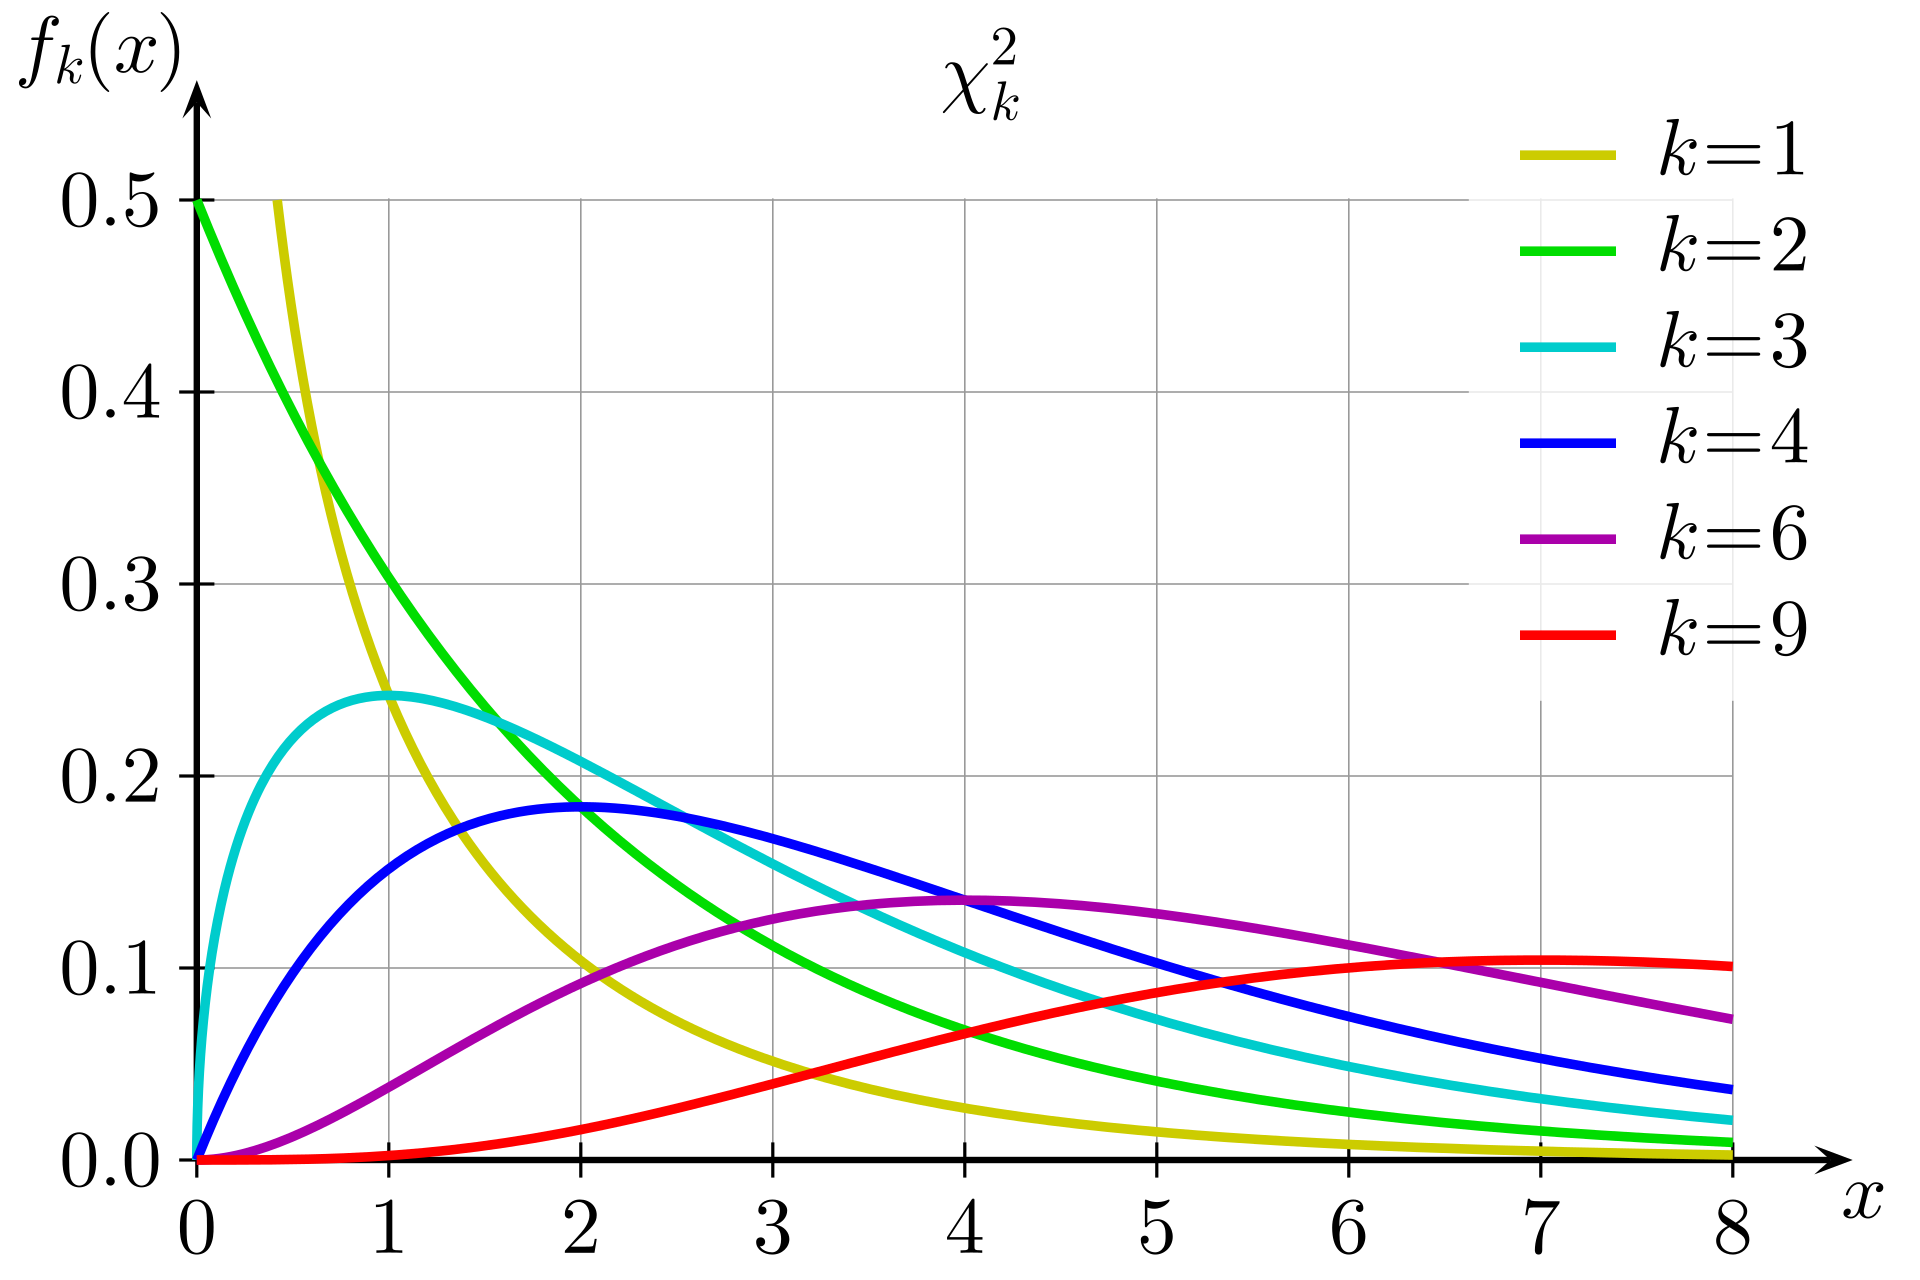
\includegraphics[
                width=\linewidth,
                height=5cm,
                keepaspectratio,
            ]{images/distributions/Chi-square_pdf.svg.png}
            \caption{Chi-squared Distribution: PDF \cite{wiki/Chi-squared_distribution}}
        \end{figure}
    \end{minipage}
    \hfill
    \begin{minipage}{0.45\linewidth}
        \begin{figure}[H]
            \centering
            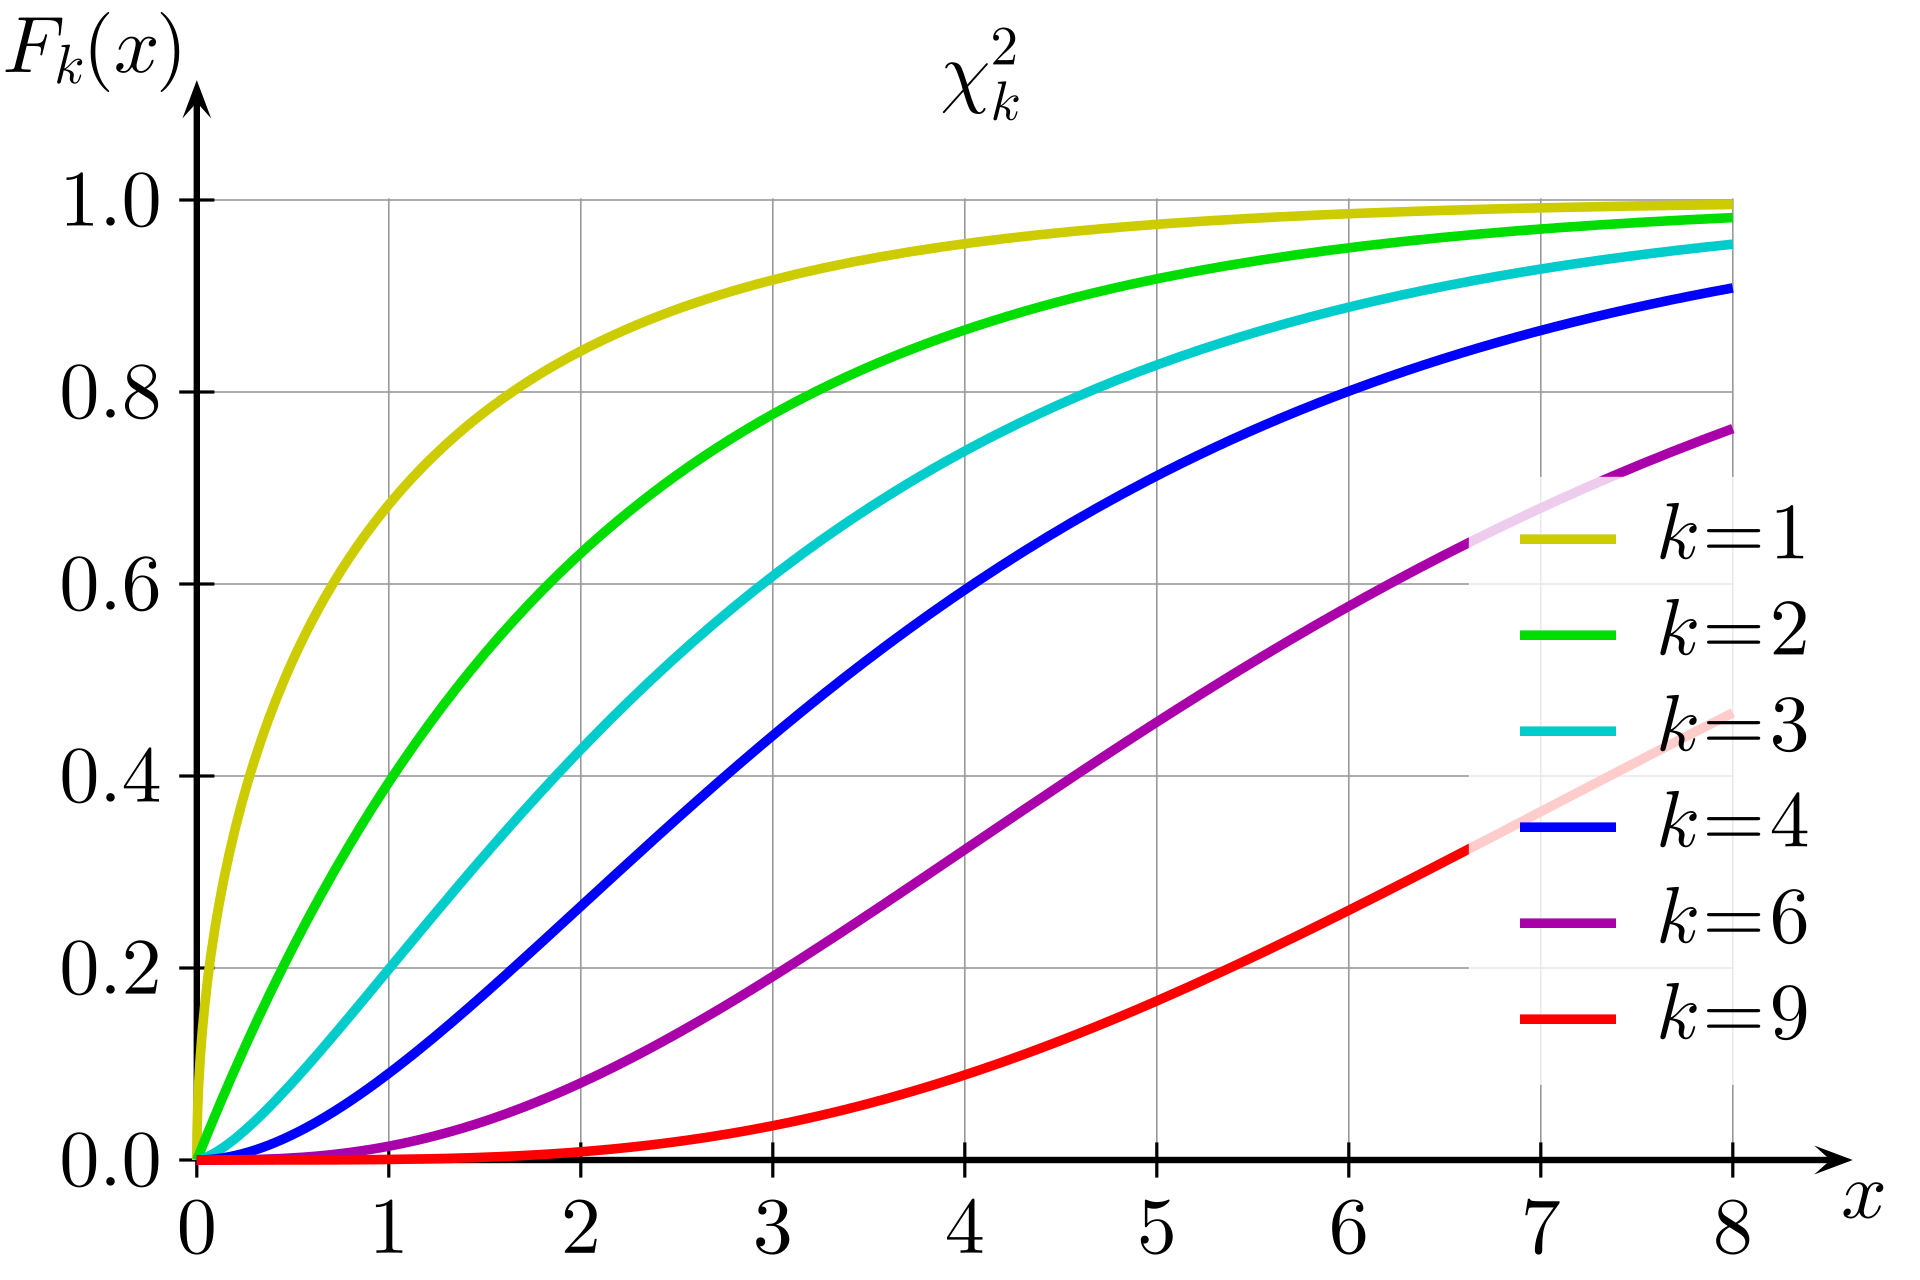
\includegraphics[
                width=\linewidth,
                height=5cm,
                keepaspectratio,
            ]{images/distributions/Chi-square_cdf.svg.png}
            \caption{Chi-squared Distribution: CDF \cite{wiki/Chi-squared_distribution}}
        \end{figure}
    \end{minipage}
    \hfill
\end{table}

\subsection{Summary}

\begin{enumerate}
    \item \textbf{Parameters}: ${\displaystyle k\in \mathbb {N} ^{*}}$ (known as "degrees of freedom")
    \hfill \cite{wiki/Chi-squared_distribution}

    \item \textbf{Support}: $  {\displaystyle x\in (0,+\infty )} $
    \hfill \cite{wiki/Chi-squared_distribution}

    \item \textbf{PDF}: $  {\displaystyle {\dfrac {1}{2^{k/2}\Gamma (k/2)}}\;x^{(k/2)-1}e^{-x/2}} $
    \hfill \cite{wiki/Chi-squared_distribution}

    \item \textbf{CDF}: $  {\displaystyle {\dfrac {1}{\Gamma (k/2)}}\;\gamma \left({\dfrac {k}{2}},\,{\dfrac {x}{2}}\right)\;} $
    \hfill \cite{wiki/Chi-squared_distribution}

    % \item \textbf{Quantile}: $  $
    % \hfill \cite{wiki/Chi-squared_distribution}

    \item \textbf{Mean}: $ k $
    \hfill \cite{wiki/Chi-squared_distribution}

    \item \textbf{Median}: $  {\displaystyle \approx k{\bigg (}1-{\dfrac {2}{9k}}{\bigg )}^{3}\;} $
    \hfill \cite{wiki/Chi-squared_distribution}

    \item \textbf{Mode}: $  {\displaystyle \max(k-2,0)\;} $
    \hfill \cite{wiki/Chi-squared_distribution}

    \item \textbf{Variance}: $  {\displaystyle 2k\;} $
    \hfill \cite{wiki/Chi-squared_distribution}

    \item \textbf{Skewness}: $  {\displaystyle {\sqrt {\dfrac{8}{k}}}\,} $
    \hfill \cite{wiki/Chi-squared_distribution}

    \item \textbf{Excess kurtosis}: $  {\displaystyle {\dfrac {12}{k}}} $
    \hfill \cite{wiki/Chi-squared_distribution}

    \item \textbf{Entropy}: $  {\displaystyle {\dfrac {k}{2}} +\log \left(2\Gamma {\Bigl (}{\dfrac {k}{2}}{\Bigr )}\right) \!+\left(1-{\dfrac {k}{2}}\right)\psi \left({\dfrac {k}{2}}\right)} $
    \hfill \cite{wiki/Chi-squared_distribution}

    % \item \textbf{Fisher information}: $  $
    % \hfill \cite{wiki/Chi-squared_distribution}

    % \item \textbf{Expected shortfall}: $  $
    % \hfill \cite{wiki/Chi-squared_distribution}

    \item \textbf{Moment-generating function (MGF)}: $  {\displaystyle (1-2t)^{-k/2}{\text{ for }}t<{\dfrac {1}{2}}\;} $
    \hfill \cite{wiki/Chi-squared_distribution}

    \item \textbf{Characteristic function (CF)}:
    $  ( 1 - 2 i t ) - k / 2 {\displaystyle (1-2it)^{-k/2}} $
    \hfill \cite{wiki/Chi-squared_distribution}

    \item \textbf{Probability-generating function (PGF)}: $  {\displaystyle (1-2\ln t)^{-k/2}{\text{ for }}0<t<{\sqrt {e}}\;} $
    \hfill \cite{wiki/Chi-squared_distribution}

    % \item \textbf{Kullback–Leibler divergence}:
    % $  $
    % \hfill \cite{wiki/Chi-squared_distribution}

    % \item \textbf{Median absolute deviation (MAD)}:
    % $  $
    % \hfill \cite{wiki/Chi-squared_distribution}
\end{enumerate}











